\documentclass[10pt,landscape,a4paper]{article}
\usepackage[utf8]{inputenc}
\usepackage[ngerman]{babel}
\usepackage[utopia,sfscaled]{mathdesign}
%\usepackage[lf,minionint]{MinionPro}
%\renewcommand{\sfdefault}{phv}
%\usepackage[lf]{MyriadPro}
\usepackage{multicol}
\usepackage[top=5mm,bottom=5mm,left=5mm,right=5mm]{geometry}
%\usepackage{hyperref}
\usepackage{lipsum}
\usepackage[framemethod=tikz]{mdframed}
%\usepackage{fancyhdr} ---> ???
\usepackage{microtype}
\usepackage{mathtools}
\usepackage[]{graphics}
\usepackage{float}

% Abs
\DeclarePairedDelimiter\abs{\lvert}{\rvert}%
\makeatletter
\let\oldabs\abs
\def\abs{\@ifstar{\oldabs}{\oldabs*}}

\renewcommand{\baselinestretch}{.8}
\pagestyle{empty}

\global\mdfdefinestyle{header}{%
	linecolor=black,linewidth=1pt,%
	leftmargin=0mm,rightmargin=0mm,skipbelow=0mm,skipabove=0mm,
}




\makeatletter
\renewcommand{\section}{\@startsection{section}{1}{5mm}%
	{.2ex}%
	{.2ex}%x
	{\sffamily\bfseries}}



\def\multi@column@out{%
	\ifnum\outputpenalty <-\@M
	\speci@ls \else
	\ifvoid\colbreak@box\else
	\mult@info\@ne{Re-adding forced
		break(s) for splitting}%
	\setbox\@cclv\vbox{%
		\unvbox\colbreak@box
		\penalty-\@Mv\unvbox\@cclv}%
	\fi
	\splittopskip\topskip
	\splitmaxdepth\maxdepth
	\dimen@\@colroom
	\divide\skip\footins\col@number
	\ifvoid\footins \else
	\leave@mult@footins
	\fi
	\let\ifshr@kingsaved\ifshr@king
	\ifvbox \@kludgeins
	\advance \dimen@ -\ht\@kludgeins
	\ifdim \wd\@kludgeins>\z@
	\shr@nkingtrue
	\fi
	\fi
	\process@cols\mult@gfirstbox{%
		%%%%% START CHANGE
		\ifnum\count@=\numexpr\mult@rightbox+2\relax
		\setbox\count@\vsplit\@cclv to \dimexpr \dimen@-1cm\relax
		%\setbox\count@\vbox to \dimen@{\vbox to 1.25cm{\header}\unvbox\count@\vss}%
		\else
		\setbox\count@\vsplit\@cclv to \dimen@
		\fi
		%%%%% END CHANGE
		\set@keptmarks
		\setbox\count@
		\vbox to\dimen@
		{\unvbox\count@
			\remove@discardable@items
			\ifshr@nking\vfill\fi}%
	}%
	\setbox\mult@rightbox
	\vsplit\@cclv to\dimen@
	\set@keptmarks
	\setbox\mult@rightbox\vbox to\dimen@
	{\unvbox\mult@rightbox
		\remove@discardable@items
		\ifshr@nking\vfill\fi}%
	\let\ifshr@king\ifshr@kingsaved
	\ifvoid\@cclv \else
	\unvbox\@cclv
	\ifnum\outputpenalty=\@M
	\else
	\penalty\outputpenalty
	\fi
	\ifvoid\footins\else
	\PackageWarning{multicol}%
	{I moved some lines to
		the next page.\MessageBreak
		Footnotes on page
		\thepage\space might be wrong}%
	\fi
	\ifnum \c@tracingmulticols>\thr@@
	\hrule\allowbreak \fi
	\fi
	\ifx\@empty\kept@firstmark
	\let\firstmark\kept@topmark
	\let\botmark\kept@topmark
	\else
	\let\firstmark\kept@firstmark
	\let\botmark\kept@botmark
	\fi
	\let\topmark\kept@topmark
	\mult@info\tw@
	{Use kept top mark:\MessageBreak
		\meaning\kept@topmark
		\MessageBreak
		Use kept first mark:\MessageBreak
		\meaning\kept@firstmark
		\MessageBreak
		Use kept bot mark:\MessageBreak
		\meaning\kept@botmark
		\MessageBreak
		Produce first mark:\MessageBreak
		\meaning\firstmark
		\MessageBreak
		Produce bot mark:\MessageBreak
		\meaning\botmark
		\@gobbletwo}%
	\setbox\@cclv\vbox{\unvbox\partial@page
		\page@sofar}%
	\@makecol\@outputpage
	\global\let\kept@topmark\botmark
	\global\let\kept@firstmark\@empty
	\global\let\kept@botmark\@empty
	\mult@info\tw@
	{(Re)Init top mark:\MessageBreak
		\meaning\kept@topmark
		\@gobbletwo}%
	\global\@colroom\@colht
	\global \@mparbottom \z@
	\process@deferreds
	\@whilesw\if@fcolmade\fi{\@outputpage
		\global\@colroom\@colht
		\process@deferreds}%
	\mult@info\@ne
	{Colroom:\MessageBreak
		\the\@colht\space
		after float space removed
		= \the\@colroom \@gobble}%
	\set@mult@vsize \global
	\fi}

\makeatother
\setlength{\parindent}{0pt}

% -- -- -- -- -- -- -- -- -- -- -- -- -- -- -- -- -- -- -- -- 
\newcommand{\header}{
	\begin{mdframed}[style=header]
		\footnotesize
		\large \textbf{DSP Cheat Sheet}
	\end{mdframed}
}
% -- -- -- -- -- -- -- -- -- -- -- -- -- -- -- -- -- -- -- -- 

%% INCLUDES
% -- -- -- -- -- -- -- -- -- -- -- -- -- -- -- -- -- -- -- -- 
\usepackage{amsmath, amsthm}
\usepackage{titlesec}
\usepackage{tikz,pgfplots,filecontents,amsmath}
\pgfplotsset{compat=1.5}

%% FORMATTING
% -- -- -- -- -- -- -- -- -- -- -- -- -- -- -- -- -- -- -- -- 
\titleformat*{\section}{\small\bfseries}
\titleformat*{\subsection}{\footnotesize\bfseries}

%% no counter for section, only subsection
\renewcommand{\thesection}{}
\renewcommand{\thesubsection}{\arabic{subsection}}
%\setcounter{secnumdepth}{1}

%% space under section
 \titlespacing\section{0pt}{12pt plus 4pt minus 2pt}{6pt plus 2pt minus 2pt}
%\titlespacing\subsection{0pt}{0pt plus 4pt minus 2pt}{0pt plus 2pt minus 2pt}
%\titlespacing\subsubsection{0pt}{12pt plus 4pt minus 2pt}{0pt plus 2pt minus 2pt}


%% COMMANDS
% -- -- -- -- -- -- -- -- -- -- -- -- -- -- -- -- -- -- -- -- 
\newcommand{\mi}{\mathrm{i}} %% roman "i"
\newcommand{\di}{i}          %% default math "i"



%% START DOCUMENT
% -- -- -- -- -- -- -- -- -- -- -- -- -- -- -- -- -- -- -- -- 
\begin{document}
	\begin{multicols*}{5}
		
		\footnotesize
		% -- -- -- -- -- -- -- -- -- -- -- -- -- -- -- -- -- -- -- --
		\section{Time Domain}
		% -- -- -- -- -- -- -- -- -- -- -- -- -- -- -- -- -- -- -- --
		
		% -- -- -- -- -- -- -- -- -- -- -- -- -- -- -- -- -- -- -- --
		\subsection{Definition}
		
		\begin{align*}
		f_s 		\;&=\; \text{sampling rate}\\
		\lambda 	\;&=\; \text{wavelength}\\
		T 			\;&=\; \text{period}\\
		\omega 		\;&=\; \text{angular frequency}
		\end{align*}
		
		
		% -- -- -- -- -- -- -- -- -- -- -- -- -- -- -- -- -- -- -- --
		\subsection{Wavelength $\lambda$}
		$$\lambda = \frac{c}{f}$$
		
		
		% -- -- -- -- -- -- -- -- -- -- -- -- -- -- -- -- -- -- -- --
		\subsection{Period $T$}
		$$T = 1\,ms = 1000\,Hz$$
		
		
		% -- -- -- -- -- -- -- -- -- -- -- -- -- -- -- -- -- -- -- --
		\subsection{Angular Frequency $\omega$}
		\begin{align*}
			\omega 	\;&=\;	 2 \pi f\\
			 		\;&=\; 	\frac{2\pi}{T}
		\end{align*}
		
		
		\begin{align*}
			\omega_0 	\;&=\;	 2 \pi T\\
						\;&=\; 	\pi \frac{f_0}{fs}
		\end{align*}
		

		% -- -- -- -- -- -- -- -- -- -- -- -- -- -- -- -- -- -- -- --
		\subsection{Unit Pulse \& Unit Step}
		unit pulse:
		\[
		\delta(n)= 
		\begin{cases}
			1,& \text{if }  n = 0\\
			\text{0 }  & \text{otherwise}
		\end{cases}
		\]
		
		unit step:
		\[
		u(n)= 
		\begin{cases}
		1,& \text{if }  n \geq 0\\
		\text{0}  & \text{otherwise}
		\end{cases}
		\]
		
		% -- -- -- -- -- -- -- -- -- -- -- -- -- -- -- -- -- -- -- --
		\subsection{Harmonic Signals}
		
		\begin{align*}
		n 		\;&=\; 		[1:t \cdot f_s] \\
				\;& \;		\\
		x[n] 	\;&=\;	 	sin(\omega_0 n + \varphi)\\
				\;&=\;   	sin(2 \pi f_0 T + \varphi)\\
				\;&=\;   	sin(2 \pi \frac{f_0}{fs}  n + \varphi)\\
				\;& \; 		\\
		x[n]	\;&=\;		e^{-\mi \omega_0 n}\\
				\;&=\;		cos(\omega_0 n) + \mi\; sin(\omega_0 n)
		\end{align*}
		
		
		% -- -- -- -- -- -- -- -- -- -- -- -- -- -- -- -- -- -- -- --
		\tiny \texttt{\textbf{DSP Cheatsheet} - \today}\\
		\tiny https://github.com/xhain/DSP\_Cheatsheet
		\vspace{1cm}
		% -- -- -- -- -- -- -- -- -- -- -- -- -- -- -- -- -- -- -- --
		
		
		% -- -- -- -- -- -- -- -- -- -- -- -- -- -- -- -- -- -- -- --
		%\vfill\null
		\columnbreak
		\footnotesize
		% -- -- -- -- -- -- -- -- -- -- -- -- -- -- -- -- -- -- -- --
		\section{Frequency Domain}
		% -- -- -- -- -- -- -- -- -- -- -- -- -- -- -- -- -- -- -- --
		
		
		% -- -- -- -- -- -- -- -- -- -- -- -- -- -- -- -- -- -- -- --
		\subsection{Definition}
		
		\begin{align*}
		f_s 		\;&=\; \text{sampling rate}\\
		\lambda 	\;&=\; \text{wavelength}\\
		T 			\;&=\; \text{period}\\
		\omega 		\;&=\; \text{angular frequency}
		\end{align*}
		
		% -- -- -- -- -- -- -- -- -- -- -- -- -- -- -- -- -- -- -- --
		\vfill\null
		\columnbreak
		% -- -- -- -- -- -- -- -- -- -- -- -- -- -- -- -- -- -- -- --
		\section{LTI Systems}
		% -- -- -- -- -- -- -- -- -- -- -- -- -- -- -- -- -- -- -- --
		
		\begin{align*}
		y[n]		\;&=\; T \{ \;x[n]\; \}
		\end{align*}
		
		\textit{Linear time-invariant systems} (LTI systems) are a class of systems used in signals and systems that are both linear and time-invariant. Linear systems are systems whose outputs for a linear combination of inputs are the same as a linear combination of individual responses to those inputs. Time-invariant systems are systems where the output does not depend on when an input was applied. These properties make LTI systems easier to represent and understand.
		
		\begin{enumerate}
			\item memory freedom
			\item causality
			\item stability (BIBO)
		\end{enumerate}
		
		
		
		% -- -- -- -- -- -- -- -- -- -- -- -- -- -- -- -- -- -- -- --
		\vfill\null
		\columnbreak
		% -- -- -- -- -- -- -- -- -- -- -- -- -- -- -- -- -- -- -- --
		\section{Filter Design}
		% -- -- -- -- -- -- -- -- -- -- -- -- -- -- -- -- -- -- -- --
		
		\subsection{In General}
		
		The lowpass general, standard form is given by
		
		\begin{align*}
			\abs{H(j \omega)} \;&=\; \abs{\frac{A_0}{1 + \epsilon^2 A_N^2 (\frac{\omega}{\omega_g})}}
		\end{align*}
		
		with the design criteria defined by
		
		\begin{figure}
			\centering
			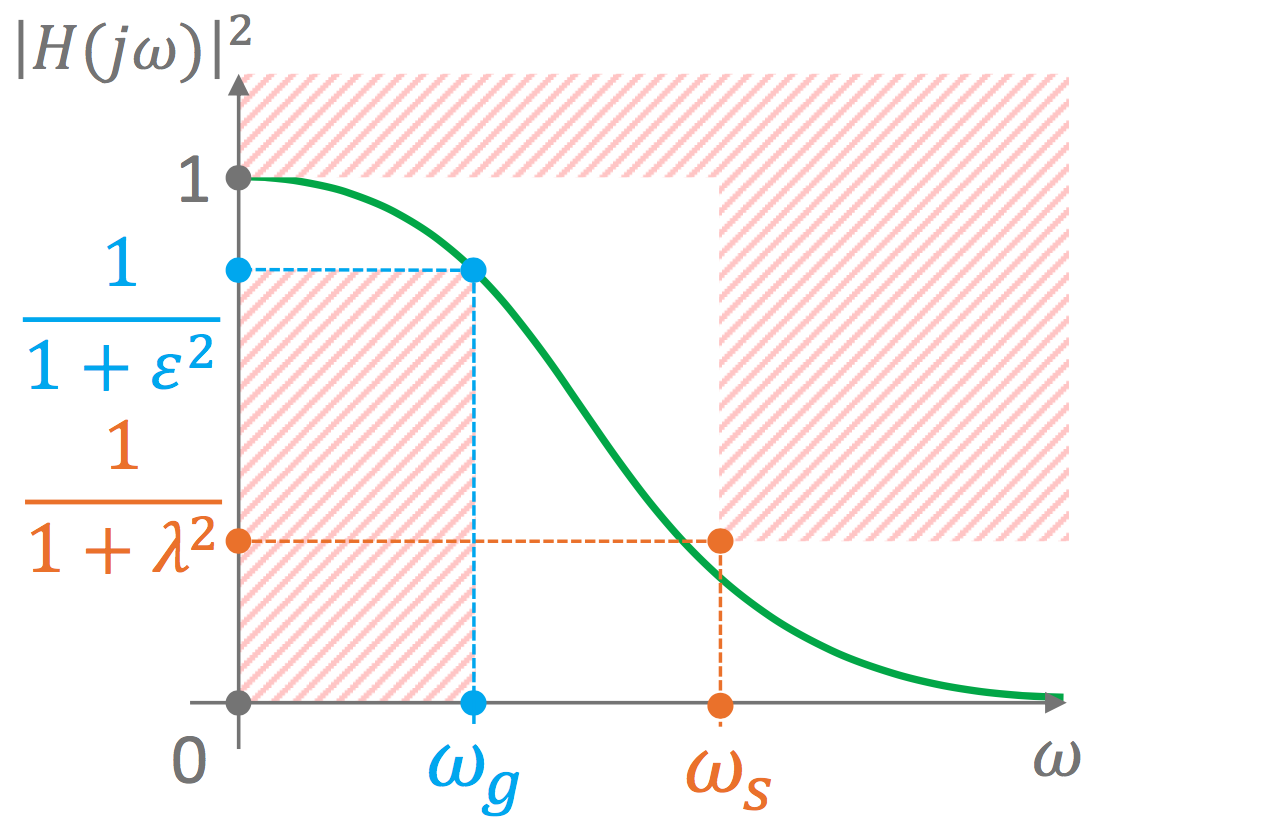
\includegraphics[width=0.7\linewidth]{img/FilterDesignCriteria.png}
			\caption{test}
			\label{fig:filterdesigncriteria}
		\end{figure}
		
		
		

	
		% -- -- -- -- -- -- -- -- -- -- -- -- -- -- -- -- -- -- -- --
		\subsection{Butterworth}
		% -- -- -- -- -- -- -- -- -- -- -- -- -- -- -- -- -- -- -- --
		The Butterworth filter is a type of signal processing filter designed to have a frequency response as flat as possible in the passband. It is also referred to as a maximally flat magnitude filter, given by
		$$ A_N(\frac{\omega}{\omega_g}) \;=\; (\frac{\omega}{\omega_g})^N $$
		
		so that
		
		\begin{align*}
		\abs{H(j \omega)} \;&=\; \abs{\frac{A_0}{1 + \epsilon^2 (\frac{\omega}{\omega_g})^{2N}}}
		\end{align*}
		
		The order $N$ is therefore given by 		
		
		\begin{align*}
		\epsilon (\frac{\omega}{\omega_g})^N 					\;&=\; \lambda \\
		\Rightarrow (\frac{\omega}{\omega_g})^N 				\;&=\; \frac{\lambda}{\epsilon} \\
		\Rightarrow N \cdot log_{10}(\frac{\omega_s}{\omega_g}) \;&=\; log_{10}(\frac{\lambda}{\epsilon})\\
		\Rightarrow N  											\;\geq\; \frac{log_{10}(\eta_s) }{ log_{10}(\frac{\omega_s}{\omega_g})}
		\end{align*}
		
		for $\eta_s = \frac{\omega_s}{\omega_g}$ and $\eta = \frac{\omega}{\omega_g}$.
		To find the poles we use
		
		\begin{align*}
		s_{\infty n}					\;&=\; \omega_g \epsilon^{-\frac{1}{N}} e^{j \frac{\pi}{2} ( \frac{(2n - 1 )}{N} +1)}
		\end{align*}
		
		and find $2N$ equidistant poles in a circle with radius $r = \omega_g \epsilon^{\frac{1}{N}}$.
			
		% -- -- -- -- -- -- -- -- -- -- -- -- -- -- -- -- -- -- -- --
		\vfill\null
		\columnbreak
		\section{}
		\subsection{Tchebychev I \& II}
		% -- -- -- -- -- -- -- -- -- -- -- -- -- -- -- -- -- -- -- --
		
		The tchebychev filter is given by
		
		\begin{align*}
		\abs{H(j \omega)} \;&=\; \abs{\frac{A_0}{1 + \epsilon^2 T_N^2 (\frac{\omega}{\omega_g})}}
		\end{align*}
		
		and uses the tchebychev polynomial $T_N$ defined by
		
		 \[
		T_N(\eta) = \left\{\begin{array}{lr}
		cos[N \cdot arccos(\eta)], & \text{for } \abs{\eta} \leq 1\\
		cosh[N \cdot arccosh(\eta)], & \text{for } \abs{\eta} > 1
		\end{array}\right\} = xy
		\]
		
		\vfill\null
		
	\end{multicols*}
\end{document}